\documentclass[10pt,a4paper]{article}
\usepackage[margin=1.8cm]{geometry}
\usepackage{amsmath,amssymb,mathtools}
\usepackage{graphicx}
\usepackage{booktabs}
\usepackage[hidelinks]{hyperref}

% ---------------------------------------------------------------- fill these in
\newcommand{\studentname}{Ruth Yegudaev}
\newcommand{\studentid}{STUDENT\_ID}
% ----------------------------------------------------------------

\graphicspath{{figures/}}
\setlength{\parindent}{0pt}
\setlength{\parskip}{0.5em}

% One experiment: \experiment{label}{title}{prediction}{observation}{explanation}
\newcommand{\experiment}[5]{%
  \subsection*{#1\quad #2}
  \textbf{Prediction.} #3\par
  \textbf{Observed.} #4\par
  \textbf{Explanation.} #5\par
}
\newcommand{\todo}[1]{\textcolor{red}{[TODO: #1]}}
\usepackage{xcolor}

\title{Visual Computing -- Exercise 2\\[2pt]\large Feature-based warping and 3D viewing}
\author{\studentname\ (ID \studentid)}
\date{Fall semester 2026--27}

\begin{document}
\maketitle


% ================================================================ PART A
\section{Part A: warping and morphing with feature lines}

Unless stated otherwise: source image \texttt{test\_image.png}, $a=1$, $b=2$, $p=0.5$.
Lines are given as $P'Q'$ (source) $\to$ $PQ$ (destination), in $(x,y)$.

\subsection{A1: one line pair}
Source line $P'=(64,128)$, $Q'=(192,128)$.

\experiment{A1a}{Three destination lines}
  {\begin{itemize}\setlength\itemsep{0pt}
     \item \emph{Translated} ($P=(84,148)$, $Q=(212,148)$): the whole picture moves right and down by 20,
       so $X'=X-(20,20)$: $(128,64)\mapsto(108,44)$ and $(160,64)\mapsto(140,44)$.
     \item \emph{Rotated} ($P=(128,64)$, $Q=(128,192)$): the picture turns $90^\circ$ clockwise about the
       midpoint $(128,128)$. The pixel $(128,64)$ is $P$ itself, so it comes from $P'=(64,128)$; $(160,64)$ is
       32 pixels to the side of the line, so it comes from $(64,96)$.
     \item \emph{Doubled} ($P=(0,128)$, $Q=(256,128)$): the picture is stretched $2\times$ along the line and
       not across it: $(128,64)\mapsto(128,64)$ and $(160,64)\mapsto(144,64)$.
   \end{itemize}}
  {Hovering over the two output pixels in the tool gave exactly the predicted source positions in all six
   cases (table below); Figure~\ref{fig:a1a} shows the results.
   The translated warp leaves a black strip at the top and at the left (positions outside the source are black);
   the rotated one turns the house on its side with the roof pointing right; in the doubled one the house is
   twice as wide and the vertical grid lines become thick and blurred.\par
   \begin{center}\small
   \begin{tabular}{lcc}\toprule
     Destination line & $X'$ at $(128,64)$ & $X'$ at $(160,64)$\\\midrule
     Translated & $(108,44)$ & $(140,44)$\\
     Rotated & $(64,128)$ & $(64,96)$\\
     Doubled & $(128,64)$ & $(144,64)$\\\bottomrule
   \end{tabular}\end{center}
   \begin{figure}[h]\centering\small
     \begin{minipage}[t]{.42\linewidth}\centering
       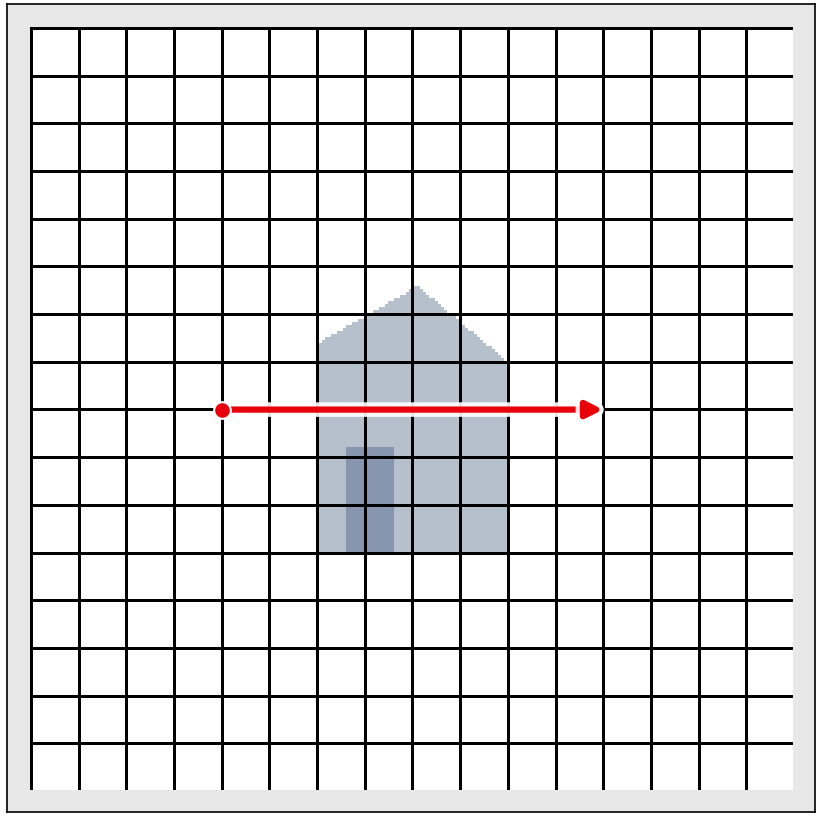
\includegraphics[width=\linewidth]{A1a_src_crop.png}\\
       source, $P'Q'=(64,128)\to(192,128)$\end{minipage}\hfill
     \begin{minipage}[t]{.42\linewidth}\centering
       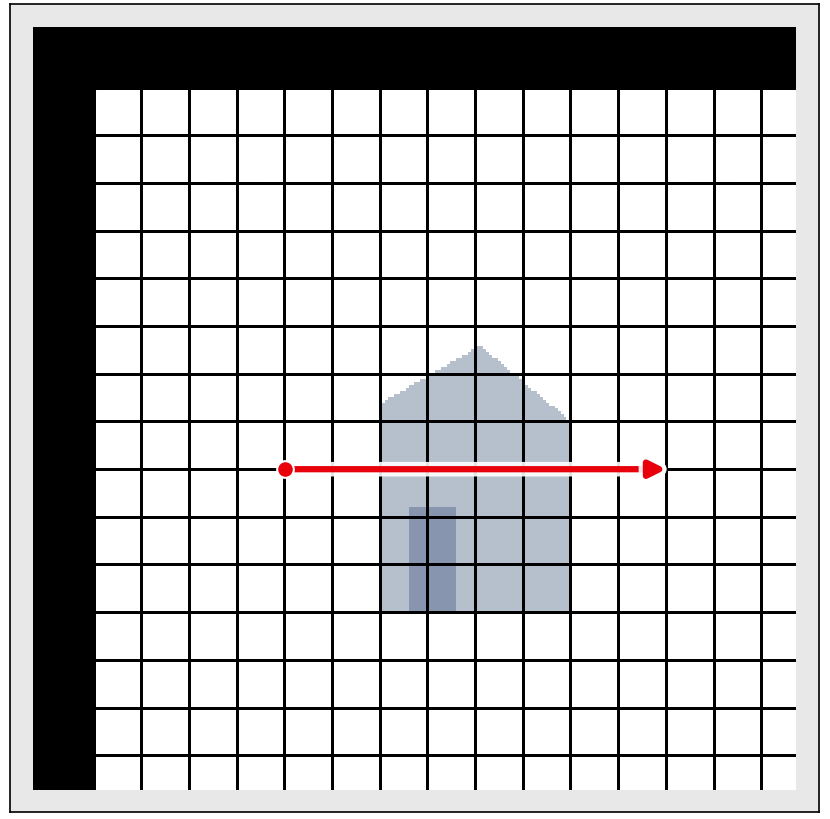
\includegraphics[width=\linewidth]{A1a_translated_out.png}\\
       translated, $PQ=(84,148)\to(212,148)$\end{minipage}\\[4pt]
     \begin{minipage}[t]{.42\linewidth}\centering
       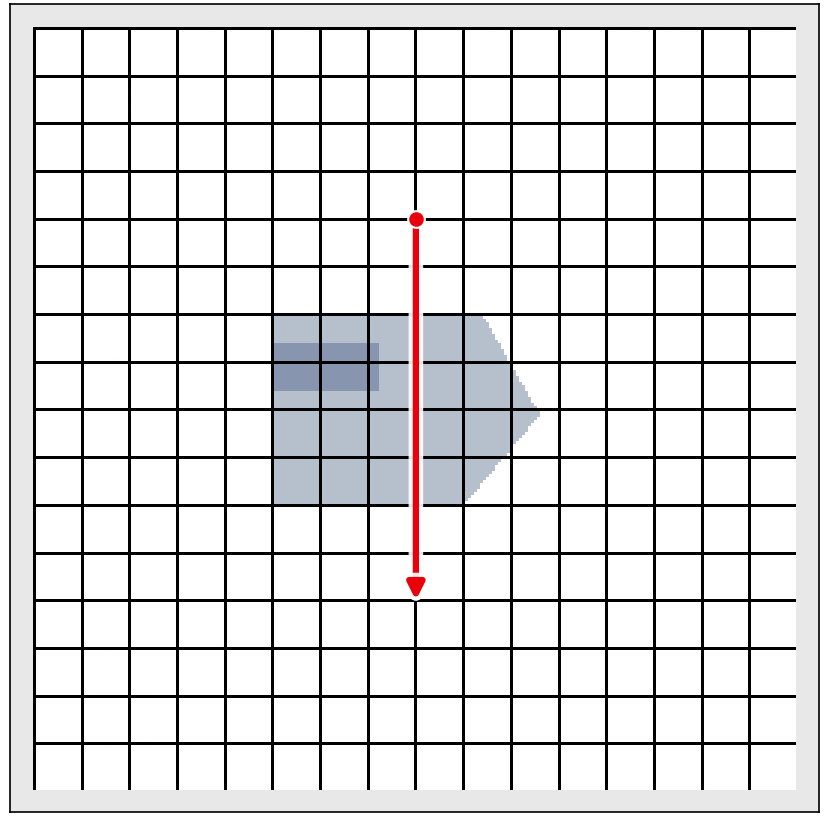
\includegraphics[width=\linewidth]{A1a_rotated_out.png}\\
       rotated, $PQ=(128,64)\to(128,192)$\end{minipage}\hfill
     \begin{minipage}[t]{.42\linewidth}\centering
       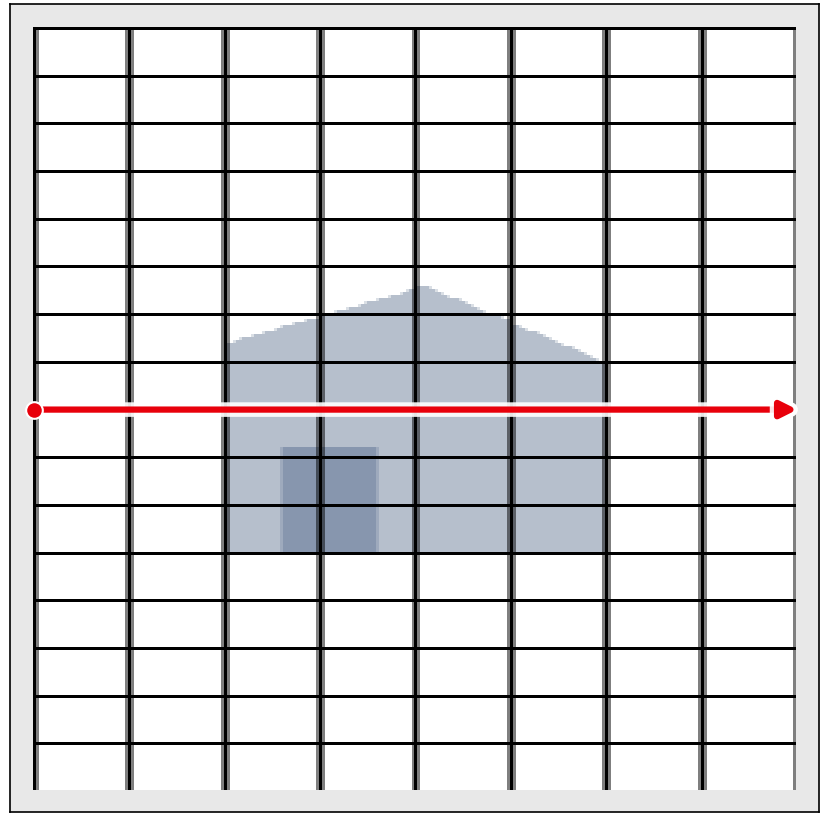
\includegraphics[width=\linewidth]{A1a_doubled_out.png}\\
       doubled, $PQ=(0,128)\to(256,128)$\end{minipage}
     \caption{A1a. The source image with its line $P'Q'$, and the three outputs with their destination
       lines $PQ$; $a=1$, $b=2$, $p=0.5$, bilinear.}\label{fig:a1a}
   \end{figure}}
  {With one line pair the warp measures each output pixel by $u$ (position along the line, as a fraction of its
   length) and $v$ (signed distance from it, in pixels), and takes the source point with the same $u$ and $v$
   relative to $P'Q'$. A translation of the line therefore translates the image, a rotation of the line rotates
   it about the line's midpoint, and doubling the length scales $u$-distances by $2$ but leaves $v$ in pixels,
   so the stretch is only along the line. The black strips and blurry vertical lines come from backward warping:
   positions outside the source are black, and magnifying by $2$ makes bilinear sampling blend neighbouring pixels.}

\experiment{A1b}{Is the warp one affine transformation?}
  {In all three cases of A1a the warp is a single affine transformation. The translated and the rotated
   warps are similarities (a translation, and a $90^\circ$ rotation about $(128,128)$). The doubled warp is
   \emph{not} a similarity: it scales $x$ by $2$ and leaves $y$ unchanged.}
  {Fitting an affine map to the source positions of all $256\times256$ output pixels leaves a maximal error
   of about $10^{-12}$ pixels in every case, so each warp is exactly affine. Written as the matrix $M$ that
   takes a source point to its output position (the matrix that \texttt{warp\_matrix} expects):
   \[
   M_{\text{transl.}}=\begin{pmatrix}1&0&20\\0&1&20\\0&0&1\end{pmatrix},\quad
   M_{\text{rot.}}=\begin{pmatrix}0&-1&256\\1&0&0\\0&0&1\end{pmatrix},\quad
   M_{\text{doubled}}=\begin{pmatrix}2&0&-128\\0&1&0\\0&0&1\end{pmatrix}.
   \]
   (The map from output to source, i.e.\ $X'$ as a function of $X$, is the inverse; for the doubled line
   $X'=(64+x/2,\;y)$.) The linear part of $M_{\text{doubled}}$ has singular values $2$ and $1$, so it is not a
   similarity; the other two have singular values $1,1$. Warping the grid image with
   \texttt{warp\_matrix}$(M)$ gives the same image as \texttt{warp\_lines} in all three cases (largest
   difference $<10^{-13}$).}
  {For one line pair, $u$ and $v$ are linear functions of $X$, and $X'=P'+u\,(Q'-P')+v\,\mathrm{perp}(Q'-P')/\|Q'-P'\|$
   is therefore an affine function of $X$. Its linear part is a rotation times a scale in the direction along
   the line (the ratio $\|Q'-P'\|/\|Q-P\|$, here $1/2$) and a scale of $1$ across it (because $v$ is measured in
   pixels). It is a similarity exactly when the two scales are equal, i.e.\ when the destination line has the
   same length as the source line, which holds for the translated and rotated lines but not for the doubled one.}

\experiment{A1c}{Effect of $a$, $b$, $p$}
  {With a single line pair, changing $a$, $b$ or $p$ should have no effect at all, because the weight $w_1$
   of the only line cancels out in the weighted average.}
  {Computing \texttt{warp\_lines} for the doubled line of A1a (source $(64,128)\to(192,128)$, destination
   $(0,128)\to(256,128)$) with ten different settings ($a\in\{0.01,1,10,100\}$, $b\in\{0,0.5,2,5\}$, $p\in\{0,0.5,1,3\}$, including
   $(a,b,p)=(100,0,3)$), the output is identical to the one for $a=1$, $b=2$, $p=0.5$: the largest difference
   over all pixels is exactly $0$.}
  {The warp is $X'=X+\sum_i w_iD_i/\sum_i w_i$. With one line, $\sum_i w_iD_i/\sum_i w_i=w_1D_1/w_1=D_1$ for
   every $w_1>0$, so $X'=X'_1$ whatever $a$, $b$ and $p$ are. These parameters only decide how the lines share
   their influence, so they matter once there are at least two lines (A2).}

\experiment{A1d}{Interpolation: magnify and shrink}
  {Source line $(64,128)\to(192,128)$. \emph{Magnify} ($P=(-64,128)$, $Q=(320,128)$, three times as long):
   with nearest neighbor each 1-pixel vertical grid line becomes a wider block with hard edges; with
   bilinear it becomes a wide band with soft, gray edges. \emph{Shrink} ($P=(110,128)$, $Q=(146,128)$):
   I expected every grid line to stay visible, just closer together, and bilinear to give a smoother row
   without gaps.}
  {Source row $y=72$ has 1-pixel dark lines at $x'=0,16,32,\dots$ (Figure~\ref{fig:a1d}).
   \emph{Magnify:} the source position is $x'=128+(x-128)/3$ and $y'=72$. Near $x=128$, nearest gives a hard
   line of width 3 pixels ($x=127,128,129$ are $0$, all others $1$), and bilinear gives a ramp
   $1,\,0.67,\,0.33,\,0,\,0.33,\,0.67,\,1$ for $x=125,\dots,131$, i.e.\ a wider and softer line.
   \emph{Shrink:} here $x'=128+3.56\,(x-128)$, so the row samples the source at steps of $3.56$ pixels.
   Both methods give exactly the same row (largest difference $0$): only the lines at $x=101,110,119,128,137,146,155$
   are drawn, 9 pixels apart, which come from $x'=32,64,\dots,224$. The lines at $x'=16,48,80,\dots$ are missing
   (so the line spacing is $9$ px instead of $4.5$ px), and outside $x=92..163$ the row is black because
   $x'$ falls outside the source. This differs from my prediction.
   \begin{figure}[h]\centering
     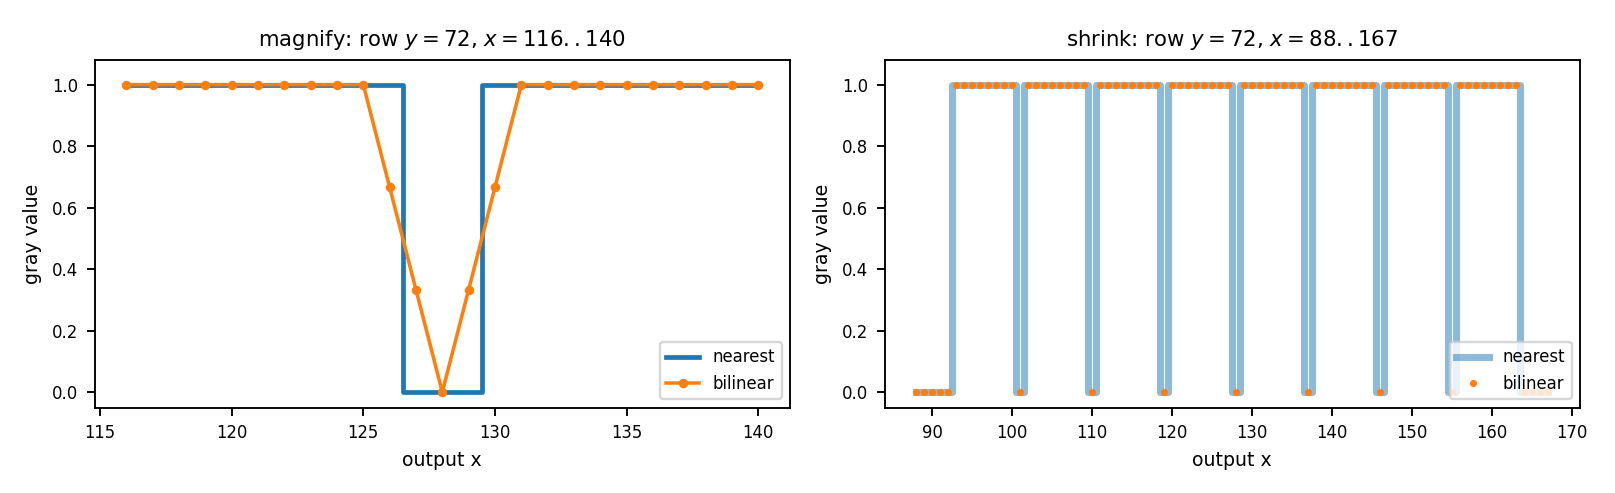
\includegraphics[width=.95\linewidth]{A1d_rows.png}
     \caption{A1d, row $y=72$ of the output for the two sampling methods. Source line $(64,128)\to(192,128)$;
       magnify $PQ=(-64,128)\to(320,128)$, shrink $PQ=(110,128)\to(146,128)$; $a=1$, $b=2$, $p=0.5$.}\label{fig:a1d}
   \end{figure}}
  {When the image is magnified, each output pixel falls between source pixels: nearest copies the closest one,
   giving hard blocks, while bilinear blends the two neighbours, giving a ramp. When the image is shrunk by about
   $3.6\times$, the output samples the source every $3.56$ pixels, which is coarser than the 1-pixel lines
   spaced 16 pixels apart, so lines that fall between two samples disappear (aliasing). Bilinear averages only the
   2 nearest pixels at a single point, not the whole $3.56$-pixel footprint, so it misses the same lines and the
   two methods agree on this row; avoiding the problem would need to low-pass filter the source first.}

\subsection{A2: two line pairs}
Source lines $(64,64)\to(192,64)$ and $(64,192)\to(192,192)$; destination: first line moved
down to $(64,96)\to(192,96)$, second unchanged.

\experiment{A2a}{Vertical displacement}
  {The pixel $(128,96)$ lies on the moved line, so it should come from about $32$ pixels higher
   ($y'-y\approx-32$). The pixel $(128,168)$ is close to the unmoved line, so its displacement should be small
   (about $-3$). The displacement at $(128,120)$, which is nearer to the moved line, should be larger in
   magnitude than at $(128,144)$, which is halfway between the two lines. Row $y=144$ should sample a straight
   line of the source, but row $y=120$ should bend.}
  {\begin{center}\small
   \begin{tabular}{lcccc}\toprule
     output pixel & $(128,96)$ & $(128,120)$ & $(128,144)$ & $(128,168)$\\\midrule
     $y'-y$ & $-32.0$ & $-28.6$ & $-16.0$ & $-3.4$\\\bottomrule
   \end{tabular}\end{center}
   For $x=128$, $x'=x$ in all four cases. Row $y=144$ samples $y'=128$ for every $x$ from $0$ to $255$,
   a straight horizontal line of the source ($y'-y=-16.0$ at $x=0$ and at $x=128$). Row $y=120$ samples
   $y'=91.4$ for $x=64,\dots,192$ but $y'=98.8$ at $x=0$ ($y'-y=-21.2$, instead of $-28.6$ at $x=128$), so it is
   a curve and not a straight line. All of this matches the prediction.}
  {The two lines pull with weights that fall with distance, so near a line the displacement is that line's
   own ($-32$ or $0$) and in between it is a mixture, shrinking from $-32$ to $0$ as $y$ goes from $96$ to $192$.
   Row $y=144$ is equally far from both lines everywhere (also at $x=0$, which is outside the lines'
   horizontal range, because both lines have the same $x$-range), so the weights stay equal and the displacement
   is always $(-32+0)/2=-16$. For row $y=120$ the weights change with $x$: at $x=0$ the distance to the nearer
   (moved) line grows from $24$ to $\sqrt{64^2+24^2}\approx 68$ while the distance to the other grows from $72$ to
   $96$, so the moved line loses influence and the displacement shrinks.}

\experiment{A2b}{Global maps from the four endpoints}
  {Correspondences: $(64,64)\to(64,96)$, $(192,64)\to(192,96)$, $(64,192)\to(64,192)$, $(192,192)\to(192,192)$.
   I predicted that only the homography reproduces the four endpoints exactly, that both global maps change
   $y$ linearly, with displacements $-32,-24,-16,-8$ at the four pixels of A2a (unlike Beier--Neely), and that
   only the affine map keeps straight lines straight. For the trapezoid (moved line shortened to
   $(96,96)\to(160,96)$) I predicted that only the homography is exact.}
  {\textbf{Rectangle.} \texttt{fit\_affine} and \texttt{fit\_homography} give the same map,
   $x_{out}=x$, $y_{out}=0.75\,y+48$, and both reproduce all four endpoints exactly (error $<10^{-12}$).
   Rows $y=120$ and $y=144$ come from the straight rows $y'=96$ and $y'=128$ of the source.
   \textbf{Trapezoid.} The affine fit
   $\begin{psmallmatrix}0.75&0&32\\0&0.75&48\\0&0&1\end{psmallmatrix}$ misses every endpoint by $16$ pixels, while
   the homography
   $\begin{psmallmatrix}0.4&-0.4&76.8\\0&0&76.8\\0&-0.003&1\end{psmallmatrix}$ is exact ($<10^{-9}$); its rows
   $y=120$ and $y=144$ also sample straight rows ($y'=115.2$ and $149.3$).
   \begin{center}\small
   \begin{tabular}{llcccc}\toprule
     configuration & method & $(128,96)$ & $(128,120)$ & $(128,144)$ & $(128,168)$\\\midrule
     rectangle & Beier--Neely & $-32.0$ & $-28.6$ & $-16.0$ & $-3.4$\\
               & affine = homography & $-32.0$ & $-24.0$ & $-16.0$ & $-8.0$\\\midrule
     trapezoid & Beier--Neely & $-32.0$ & $-25.9$ & $-10.7$ & $-1.8$\\
               & affine & $-32.0$ & $-24.0$ & $-16.0$ & $-8.0$\\
               & homography & $-32.0$ & $-4.8$ & $+5.3$ & $+5.7$\\\bottomrule
   \end{tabular}\end{center}
   Values are $y'-y$ at the four pixels of A2a. Beier--Neely reproduces the endpoints to within $0.01$ pixel,
   but rows $y=120$ and $y=144$ of its output sample the source along the curves $y'\in[94.1,109.7]$ and
   $y'\in[133.3,137.4]$ in the trapezoid case. Two predictions were wrong: in the rectangle case the
   affine map is also exact, and the homography keeps straight lines straight as well.}
  {In the rectangle case the correspondences are the map $y\mapsto0.75y+48$, which is affine, so both fits are
   exact and identical, and the displacement changes evenly with $y$, whereas Beier--Neely's weights make it
   change fast near the two lines and slowly between them. Affine maps and homographies both send straight
   lines to straight lines (a homography only loses parallelism), while the Beier--Neely warp, being a weighted
   mixture of per-line maps, does not. A trapezoid is not an affine image of a rectangle (6 degrees of freedom,
   not enough), so the affine least-squares fit leaves errors, but the homography has 8 degrees of freedom and
   hits four points exactly, at the price of a perspective stretch that even changes the sign of the
   displacement at $y=144$.}

\experiment{A2c}{Morph of two faces}
  {The morph should have much less ghosting than the plain cross-dissolve, but not none. The doubling should
   remain where I drew no lines (top of the head and hair, background, shoulders), because no line pulls the
   pixels there.}
  {Images \texttt{morph\_c.jpg} (image~0) and \texttt{morph\_d.jpg} (image~1), $384\times512$, with
   nine line pairs (Figure~\ref{fig:a2c}); $a=1$, $b=2$, $p=0.5$.
   In the cross-dissolve every feature appears twice (two pairs of eyes, the glasses over the man's
   eyebrows, his beard over her chin). In the morph at $t=0.5$ the eyes, nose, mouth and face edges coincide,
   but doubling remains in the hair at the top of the head, the background lights, the collar and shoulders,
   and the glasses are a little distorted. Measured as the mean absolute grey-level difference between the two
   aligned images (cross-dissolve $\to$ morph): whole image $0.221\to0.213$, eyes and nose region
   $0.174\to0.119$, mouth $0.209\to0.204$, hair $0.179\to0.175$, left background $0.163\to0.164$, shoulders
   $0.300\to0.345$. So the improvement is large only close to the lines, and the overall improvement is much
   smaller than I predicted.
   \begin{figure}[h]\centering
     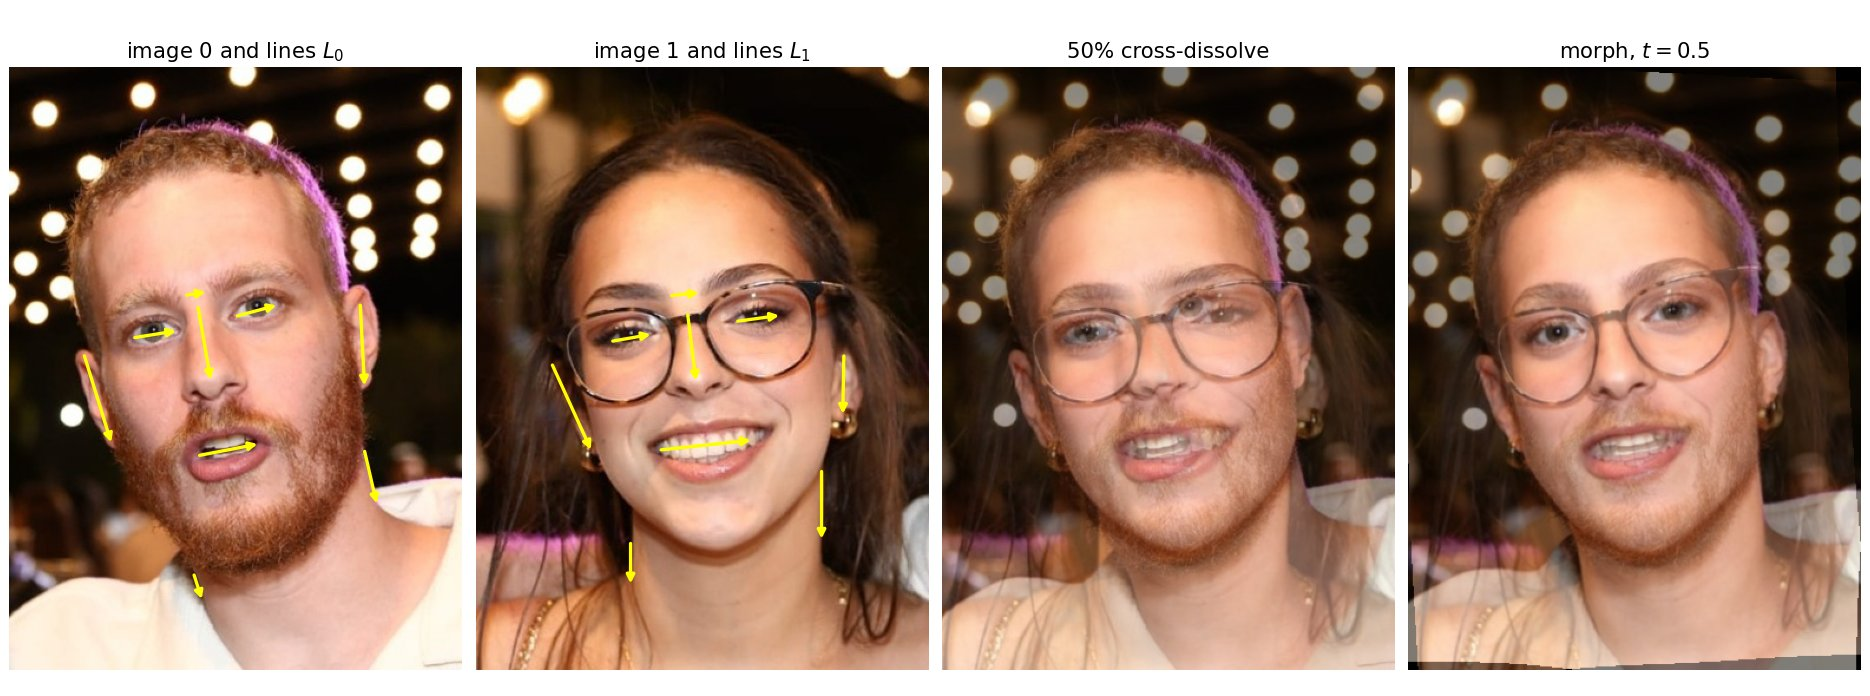
\includegraphics[width=\linewidth]{A2c_morph.jpg}
     \caption{A2c. The two images with their lines, the 50\% cross-dissolve and the morph at $t=0.5$.
       $a=1$, $b=2$, $p=0.5$.\\[2pt]
       \footnotesize
       $L_0$: (157,330)$\to$(214,319), (102,230)$\to$(145,223), (189,212)$\to$(230,201), (300,322)$\to$(312,374),
       (155,427)$\to$(164,455), (297,198)$\to$(301,274), (62,241)$\to$(87,322), (146,194)$\to$(170,190),
       (159,200)$\to$(171,269).
       $L_1$: (153,325)$\to$(237,316), (112,233)$\to$(152,226), (218,216)$\to$(261,210), (293,339)$\to$(293,404),
       (131,400)$\to$(131,442), (312,241)$\to$(311,298), (63,249)$\to$(99,328), (162,194)$\to$(193,191),
       (179,206)$\to$(187,270).}\label{fig:a2c}
   \end{figure}}
  {Each output pixel is moved by a weighted average of the displacements of the lines, with weights that fall off
   with the distance, so only pixels near a line are aligned: the eyes, nose and face edges line up, while
   hair, background and shoulders have no line nearby and stay misaligned (the shoulders even get slightly
   worse, since the lines' displacements are extrapolated there). Some content exists in only one photo (the
   glasses, the beard, the man's lights), so no choice of lines can match it. The cross-dissolve moves nothing
   and doubles every feature that differs in position.}

\subsection{A3: crossing lines}
\experiment{A3}{Uniform scaling by 2 about $C$?}
  {The warp scales by $2$ about $C$ only along the two lines, and not elsewhere. The pixel $(140,128)$, which lies
   on the horizontal line, should come from about $(134,128)$ ($=C+(X-C)/2$). For $(140,140)$, which is off both
   lines, I predicted $(134,134)$, as for a uniform scaling.}
  {Destination lines $(96,128)\to(160,128)$ and $(128,96)\to(128,160)$, source lines $(112,128)\to(144,128)$ and
   $(128,112)\to(128,144)$, $a=1$, $b=2$, $p=0.5$.
   \begin{center}\small
   \begin{tabular}{lccc}\toprule
     output pixel & uniform scaling by 2 & Beier--Neely & each line alone\\\midrule
     $(140,128)$ & $(134,128)$ & $(134.04,128)$ & $(134,128)$, $(140,128)$\\
     $(140,140)$ & $(134,134)$ & $(137,137)$ & $(134,140)$, $(140,134)$\\\bottomrule
   \end{tabular}\end{center}
   So the first prediction was right and the second was wrong. The warp is not a uniform scaling: for
   instance $(110,110)$ comes from $(114.5,114.5)$ instead of $(119,119)$, and $(140,160)$ from
   $(139.2,146.1)$ instead of $(134,144)$; the largest difference from the uniform scaling within
   $\pm50$ pixels of $C$ is about $18$ pixels.}
  {The scaling by $2$ happens only in the direction along each line, because $u$ is measured relative to the line's
   length, whereas the distance $v$ across a line is in pixels and is not scaled. On the horizontal line the
   weight of the horizontal line is overwhelming ($\mathrm{dist}=0$ against $12$ for the vertical line), so
   $(140,128)$ gets the horizontal line's answer $(134,128)$, which happens to equal the uniform scaling. At
   $(140,140)$ both lines are $12$ pixels away and have equal weights, and each line scales only one coordinate
   ($(134,140)$ and $(140,134)$), so the average is $(137,137)$ and not $(134,134)$.}

% ================================================================ PART B
\section{Part B: 3D transformations, rotations and viewing}

Key step $15^\circ$ and a reset (\texttt{r}) before each run, unless stated otherwise.

\experiment{B1}{Order of transformations}
  {After $T(0,0,-3)R_y(90^\circ)M_0$ the center is at $(0,0,-5)$ (rotate $(2,0,0)$ to $(0,0,-2)$ first, then shift),
   and after $R_y(90^\circ)T(0,0,-3)M_0$ it is at $(-3,0,-2)$ (shift to $(2,0,-3)$, then rotate about the world
   origin). I was not sure about the nose direction. The rotation about the airplane's own vertical axis is
   $M_0R_y(90^\circ)=T(2,0,0)R_y(90^\circ)T(-2,0,0)M_0$.}
  {With the matrices computed from \texttt{translate} and \texttt{rotate}:
   \begin{center}\small
   \begin{tabular}{lcc}\toprule
     matrix & center & nose direction\\\midrule
     $M_0$ & $(2,0,0)$ & $+z$\\
     $T(0,0,-3)R_y(90^\circ)M_0$ & $(0,0,-5)$ & $+x$\\
     $R_y(90^\circ)T(0,0,-3)M_0$ & $(-3,0,-2)$ & $+x$\\
     $T(2,0,0)R_y(90^\circ)T(-2,0,0)M_0$ & $(2,0,0)$ & $+x$\\\bottomrule
   \end{tabular}\end{center}
   \begin{figure}[h]\centering
     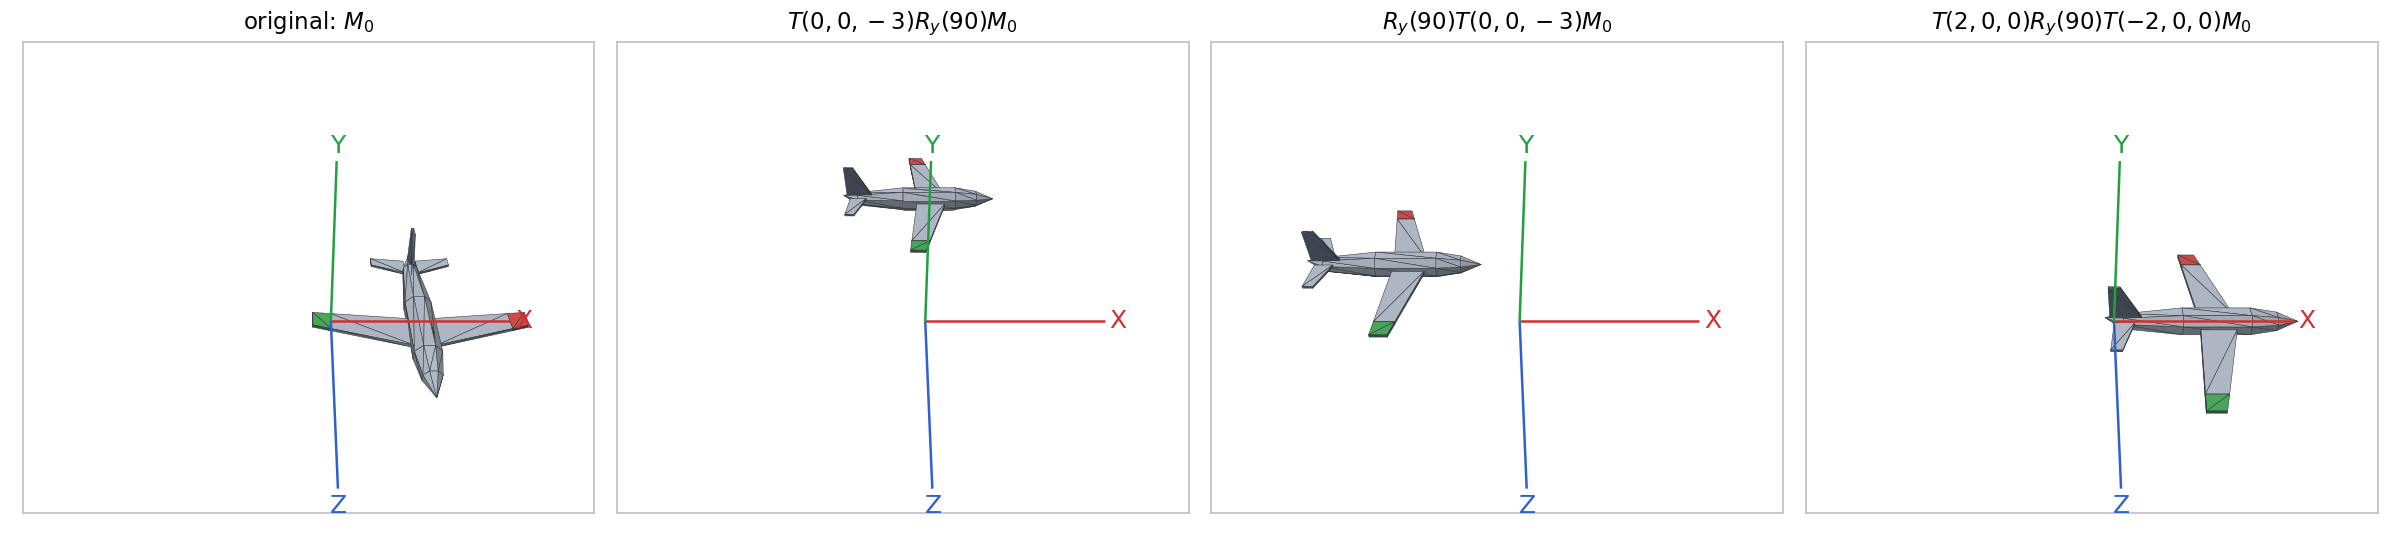
\includegraphics[width=\linewidth]{B1_strip.png}
     \caption{B1, seen from above and in front (camera at $(-0.5,9,9)$ looking at $(-0.5,0,-1.5)$, fovy $45^\circ$),
       with the world axes $X$, $Y$, $Z$: the original and the three results.}\label{fig:b1}
   \end{figure}}
  {A product acts on a point from right to left, so the rotation $R_y(90^\circ)$ turns about the world origin
   whatever comes before it: in the first product it turns $M_0$ alone, and the shift is applied afterwards,
   while in the second the shifted airplane swings around the origin to a different place. The nose ends along
   $+x$ in both cases, since a translation does not change a direction and $R_y(90^\circ)$ sends $+z$ to $+x$.
   To turn the airplane in place, the rotation has to come first in the airplane's own frame (or be conjugated
   by the translation to the center), so that its center stays at $(2,0,0)$.}

\experiment{B2a}{Rotations about world axes and object axes}
  {\todo{}}
  {\todo{Euler angles and quaternion at the end of each run}}
  {\todo{}}

\experiment{B2b}{Gimbal lock}
  {\todo{}}
  {\todo{}}
  {\todo{}}

\experiment{B3}{Interpolating rotations}
  {\todo{}}
  {\todo{axis and angle of the Euler interpolation at $t=0.25,0.5,0.75$; quaternion of key 1}}
  {\todo{}}

\experiment{B4a}{The pipeline in reverse: the image center}
  {\todo{$o$ and $d$ for $(400,300)$ in the start view; where a click there moves the airplane}}
  {\todo{}}
  {\todo{}}

\experiment{B4b}{Rays of the four corners}
  {\todo{}}
  {\todo{perspective and orthographic cases}}
  {\todo{}}

\experiment{B5a}{Chase camera: what is fixed in the image}
  {\todo{}}
  {\todo{$VM$ for two different poses}}
  {\todo{points vs.\ directions in \texttt{look\_at}}}

\experiment{B5b}{Chase camera: key behaviour}
  {\todo{}}
  {\todo{}}
  {\todo{}}

\experiment{B6a}{Find the bug: the three images}
  {\todo{}}
  {\todo{function and error for each of \texttt{bug1.png}, \texttt{bug2.png}, \texttt{bug3.png}; reproduced images}}
  {\todo{}}

\experiment{B6b}{Images 1 and 2}
  {\todo{}}
  {\todo{}}
  {\todo{why the shading differs}}

\experiment{B6c}{World-axes mode turns about the object's axes}
  {\todo{}}
  {\todo{which function, which error}}
  {\todo{}}

\end{document}
